\documentclass[11pt, a4paper]{MATH2023}
\usepackage{fancyhdr}
\usepackage{setspace}
\usepackage{amsmath,mathrsfs}
\usepackage{multicol}
\usepackage{amssymb}
\usepackage{graphicx}
\usepackage{caption}
\usepackage{subcaption}
\usepackage{xcolor}
\usepackage{enumitem}
\usepackage{tikz}
\usepackage{mathtools}
\usetikzlibrary{matrix}
\usepackage[normalem]{ulem}
\usepackage{multirow}
\usepackage[linesnumbered, ruled, boxed]{algorithm2e}
\SetKwRepeat{Do}{do}{while}
\newcommand{\eg}{\textbf{[Example.] }}
\newcommand{\sol}{\textbf{[Solution.] }}
\newcommand{\ii}{{\bf i}}
\newcommand{\jj}{{\bf j}}
\newcommand{\kk}{{\bf k}}
\newcommand{\rr}{{\bf r}}
\newcommand{\FF}{{\bf F}}
\renewcommand{\div}{{\rm div\ }}
\newcommand{\curl}{{\rm curl\ }}
\newcommand{\pt}{\partial}


\title{Chapter 15}
\subtitle{Vector Field}

\begin{document}
\begin{spacing}{1.3}

    \section{Intro. to Vector Field}

    So far, we have learned two kinds of functions involving vector: 
    \begin{itemize}
        \item ${\bf r}(t)=x(t){\bf i}+y(t){\bf j}+z(t){\bf k}$: for each $t$, provides a {\it position} vector 
        $<x(t), y(t), z(t)>$, so this is a (parametric) curve.
        \item $z=f({\bf r})=f(x_1,x_2,\cdots,x_n)$: for a given vector ${\rm r}$, this gives a real number,
        so this is a function of {\it several variables}. This is also a {\bf scalar field} since for 
        any point ${\bf r}$ in {\bf field}, it gives a scalar value. 
    \end{itemize}
    Now we are looking at {\bf vector-valued} function ${\bf F}$ of a vector ${\bf r}$, i.e., ${\bf F(r)}$.
    This is a {\bf vector field}, which means for any point ${\bf r}$ in {\bf field}, it gives a vector 
    ${\bf F(r)}$. 

    You can consider a world map showing the {\it speed} and {\it direction} of wind.
    \begin{center}
        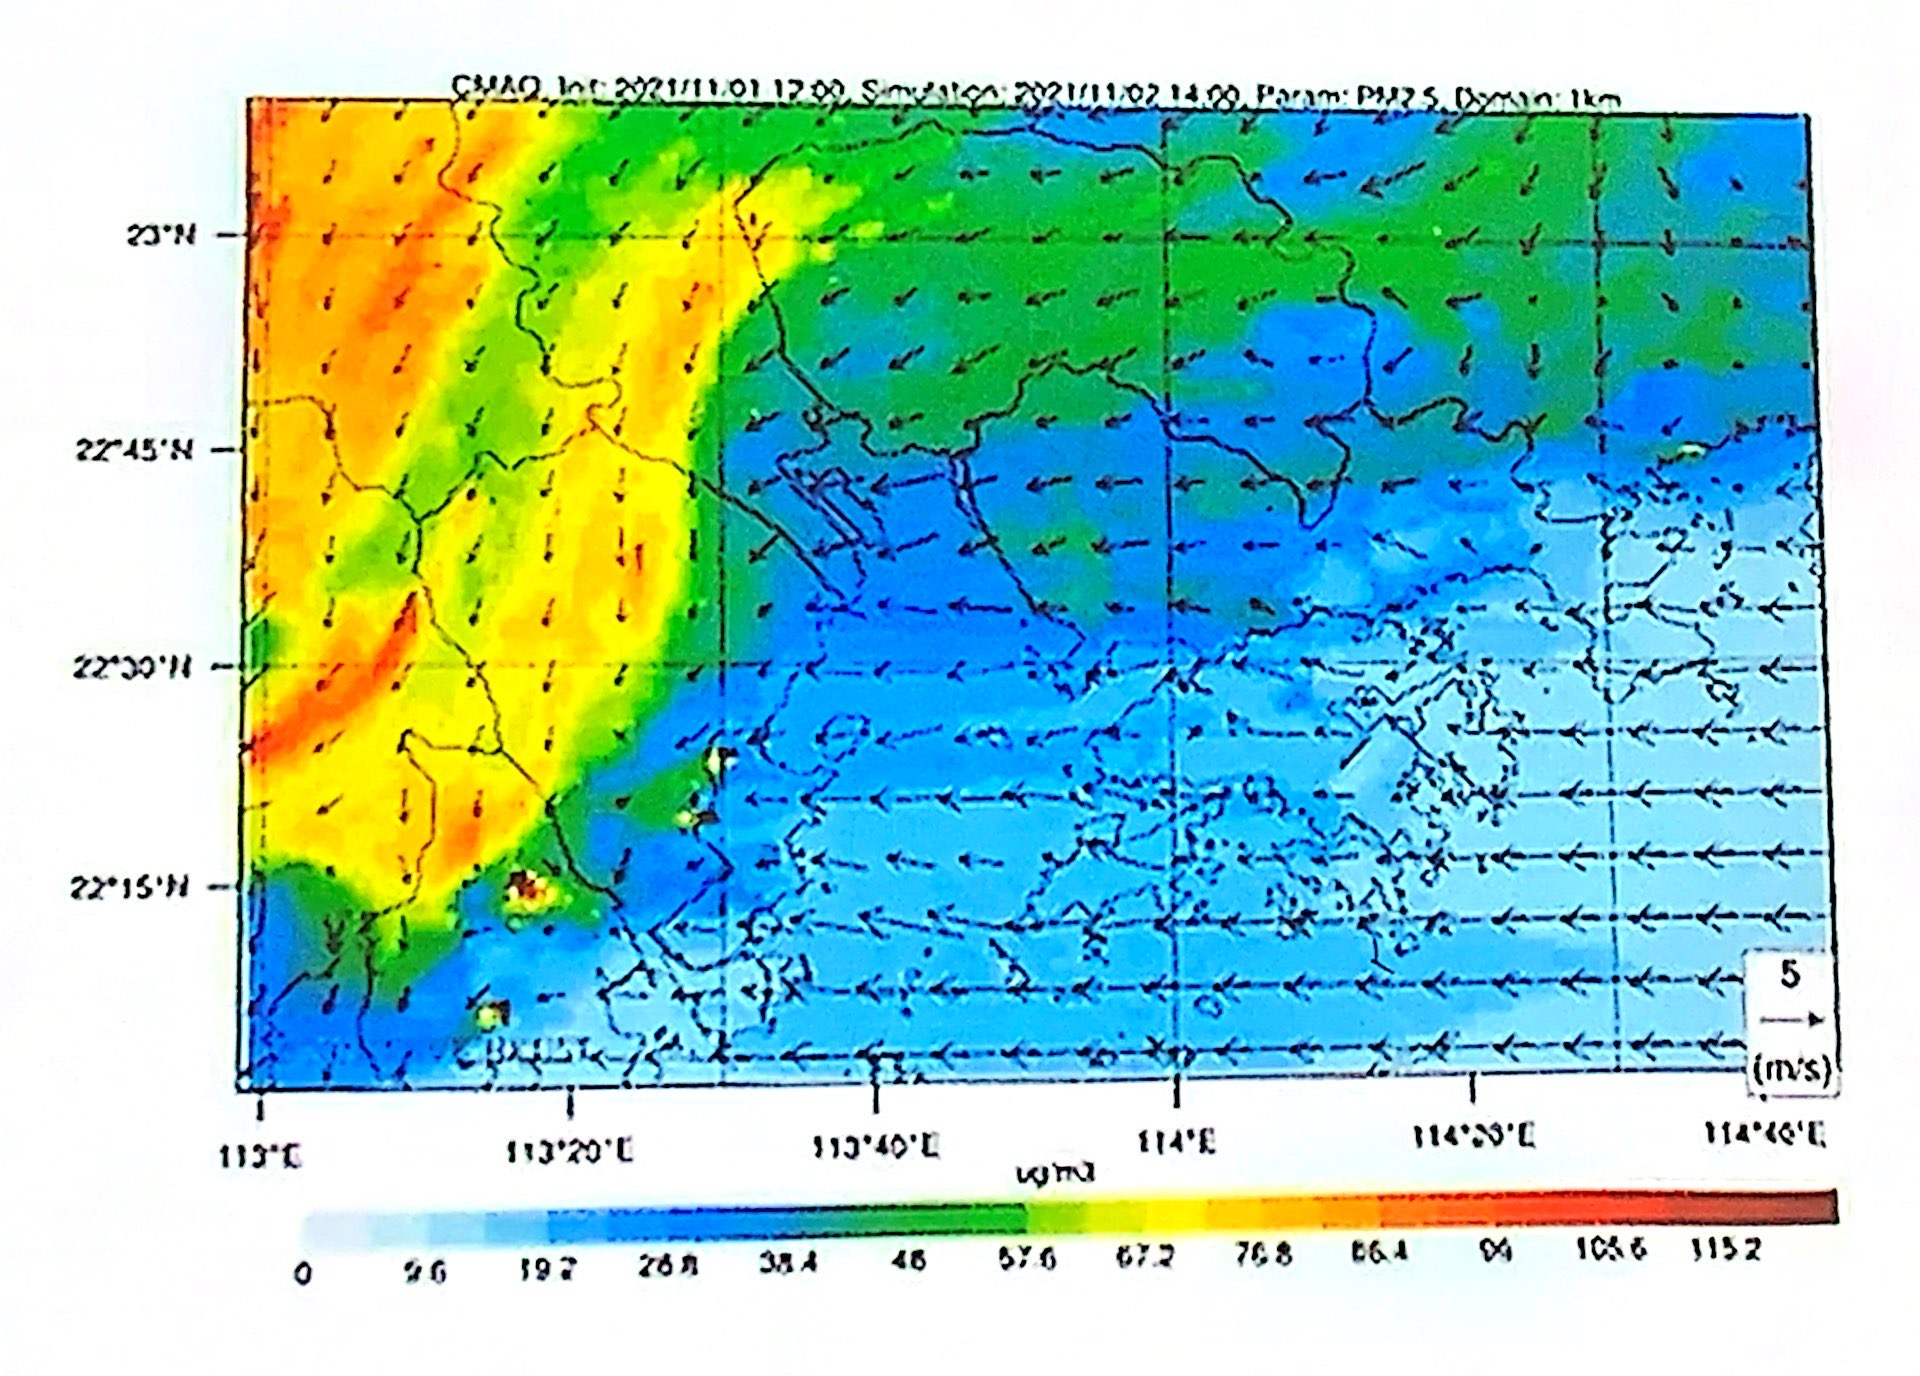
\includegraphics[scale=0.17]{images/Ch15-wind.JPG}
    \end{center}

    You can see that in a 2D map(like above), if we put a vector on each point, the vector must have 
    same dimension as the map, i.e., all vectors must also be 2D vectors.
    $${\bf F(r)}=\left\{
        \begin{array}{lll}
            (F_1({\bf r}), F_2({\bf r})) & {\bf r}=(x,y) & {\blue 2D}\\
            (F_1({\bf r}), F_2({\bf r}), F_3({\bf r})) & {\bf r}=(x,y,z) & {\blue 3D}\\
            (F_1({\bf r}), F_2({\bf r}), \cdots, F_n({\bf r})) & {\bf r}=(x_1, x_2,\cdots, x_n) & {\blue nD}
        \end{array}\right.$$
    {\bf Summary:} {\it dimension of ${\bf F}$ must be the same as ${\bf r}$.}

    \eg Assume a vector field: ${\bf F}(x,y)=\dfrac{y\ii -x\jj}{\sqrt{x^2+y^2}}$.

    \sol Notice that $||{\bf F}||=\dfrac{y^2}{x^2+y^2}+\dfrac{x^2}{x^2+y^2}=1$, all vectors 
    ${\bf F}(x,y)$ are unit vectors. Moreover, let ${\bf r}=(x,y)$, then ${\bf r}\cdot {\bf F}=0$,
    so ${\bf r}\bot {\bf F}$.

    So all vectors are unit vectors tangent to circles centered at the origin with radius $\sqrt{x^2+y^2}$.
    \begin{center}
        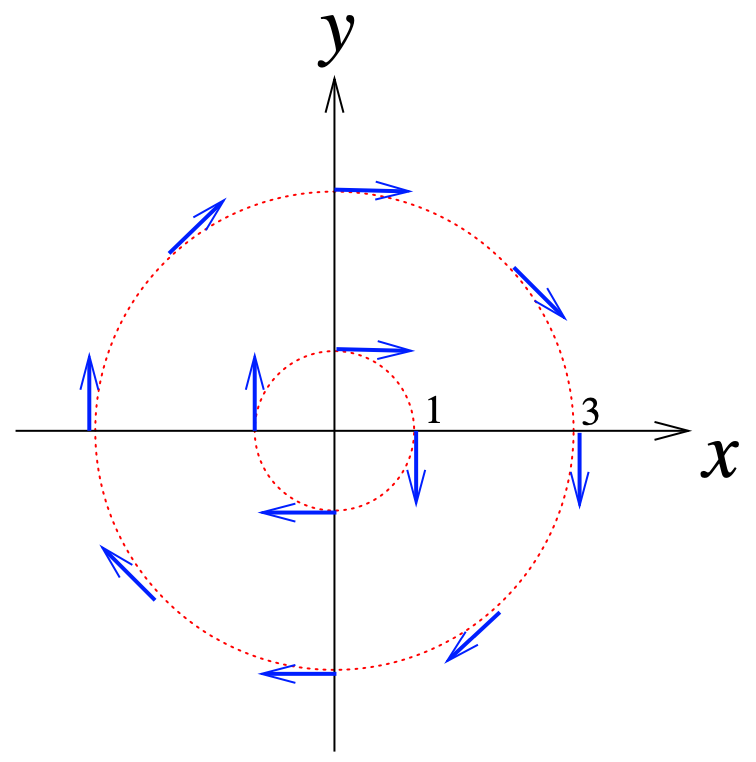
\includegraphics[scale=0.4]{images/Ch15-ex1.2.png}
    \end{center}

    \newpage
    \section{Divergence and Curl}

    Recall that the {\bf gradient operator} is a {\it vector operator}:
    $$\nabla =\left(\frac{\pt}{\pt x}, \frac{\pt}{\pt y}, \frac{\pt}{\pt z}\right)\qquad {\blue \rm (a\ vector)}$$

    If $\FF (\rr)=F_1(\rr)\ii +F_2(\rr) \jj +F_3(\rr) \kk$, then we define: 
    \begin{itemize}
        \item {\bf divergence} of $\FF$, written $\div \FF$: 
        $$
        \operatorname{div} \mathbf{F}=\nabla \cdot \mathbf{F}=\frac{\partial F_1}{\partial x}+\frac{\partial F_2}{\partial y}+\frac{\partial F_3}{\partial z}
        $$
        \item {\bf curl} of $\FF$, written $\curl \FF$: 
        $$
        \operatorname{curl} \mathbf{F}=\nabla \times \mathbf{F}=\left|\begin{array}{ccc}
        \mathbf{i} & \mathbf{j} & \mathbf{k} \\
        \dfrac{\partial}{\partial x} & \dfrac{\partial}{\partial y} & \dfrac{\partial}{\partial z} \\
        F_1 & F_2 & F_3
        \end{array}\right|=\left(\frac{\partial h}{\partial y}-\frac{\partial g}{\partial z}\right) \mathbf{i}-\left(\frac{\partial h}{\partial x}-\frac{\partial f}{\partial z}\right) \mathbf{j}+\left(\frac{\partial g}{\partial x}-\frac{\partial f}{\partial y}\right) \mathbf{k}
        $$
    \end{itemize}

    \vspace{0.2in}
    {\blue This example shows basic computation of {\bf divergence} and {\bf curl}.}

    \eg Let $\mathbf{r}=x \mathbf{i}+y \mathbf{j}+z \mathbf{k}$ and $\mathbf{u}=a \mathbf{i}+b \mathbf{j}+c \mathbf{k}$, where $a, b$ and $c$ are constants, show that

    (a) $\nabla \cdot \mathbf{r}=3$\\
    (b) $\nabla \times \mathbf{r}=\mathbf{0}$\\
    (c) $\nabla \cdot(\mathbf{u} \times \mathbf{r})=0$\\
    (d) $\nabla \times(\mathbf{u} \times \mathbf{r})=2 \mathbf{u}$.

    \sol 
    (a) $\disp \nabla \cdot \mathbf{r}=\left(\mathbf{i} \frac{\partial}{\partial x}+\mathbf{j} \frac{\partial}{\partial y}+\mathbf{k} \frac{\partial}{\partial z}\right) \cdot(x \mathbf{i}+y \mathbf{j}+z \mathbf{k})=
    \frac{\partial x}{\partial x}+\frac{\partial y}{\partial y}+\frac{\partial z}{\partial z}=3$

    (b) $\disp \nabla \times \mathbf{r}=\left|\begin{array}{ccc}
            \mathbf{i} & \mathbf{j} & \mathbf{k} \\ 
            \frac{\partial}{\partial x} & \frac{\partial}{\partial y} & \frac{\partial}{\partial z} \\ 
            x & y & z
        \end{array}\right|=\mathbf{0}$

    (c) $\disp \mathbf{u} \times \mathbf{r}=\left|\begin{array}{ccc}
            \mathbf{i} & \mathbf{j} & \mathbf{k} \\ 
            a & b & c \\ 
            x & y & z
        \end{array}\right|=(b z-c y) \mathbf{i}-(a z-c x) \mathbf{j}+(a y-b x) \mathbf{k}$

    $\disp \therefore \nabla \cdot(\mathbf{u} \times \mathbf{r})=\frac{\partial}{\partial x}(b z-c y)-\frac{\partial}{\partial y}(a z-c x)+\frac{\partial}{\partial z}(a y-b x)=0$

    (d) $\disp \nabla \times(\mathbf{u} \times \mathbf{r})=\left|\begin{array}{ccc}\mathbf{i} & \mathbf{j} & \mathbf{k} \\ \frac{\partial}{\partial x} & \frac{\partial}{\partial y} & \frac{\partial}{\partial z} \\ b z-c y & -a z+c x & a y-b x\end{array}\right|=2(a \mathbf{i}+b \mathbf{j}+c \mathbf{k})=2 \mathbf{u}$

\end{spacing}
\end{document}
